\documentclass{standalone}
\usepackage{tikz}
\usetikzlibrary{patterns, positioning}
\usepackage[sfdefault]{ClearSans} %% option 'sfdefault' activates Clear Sans as the default text font
\usepackage[T1]{fontenc}

\begin{document}
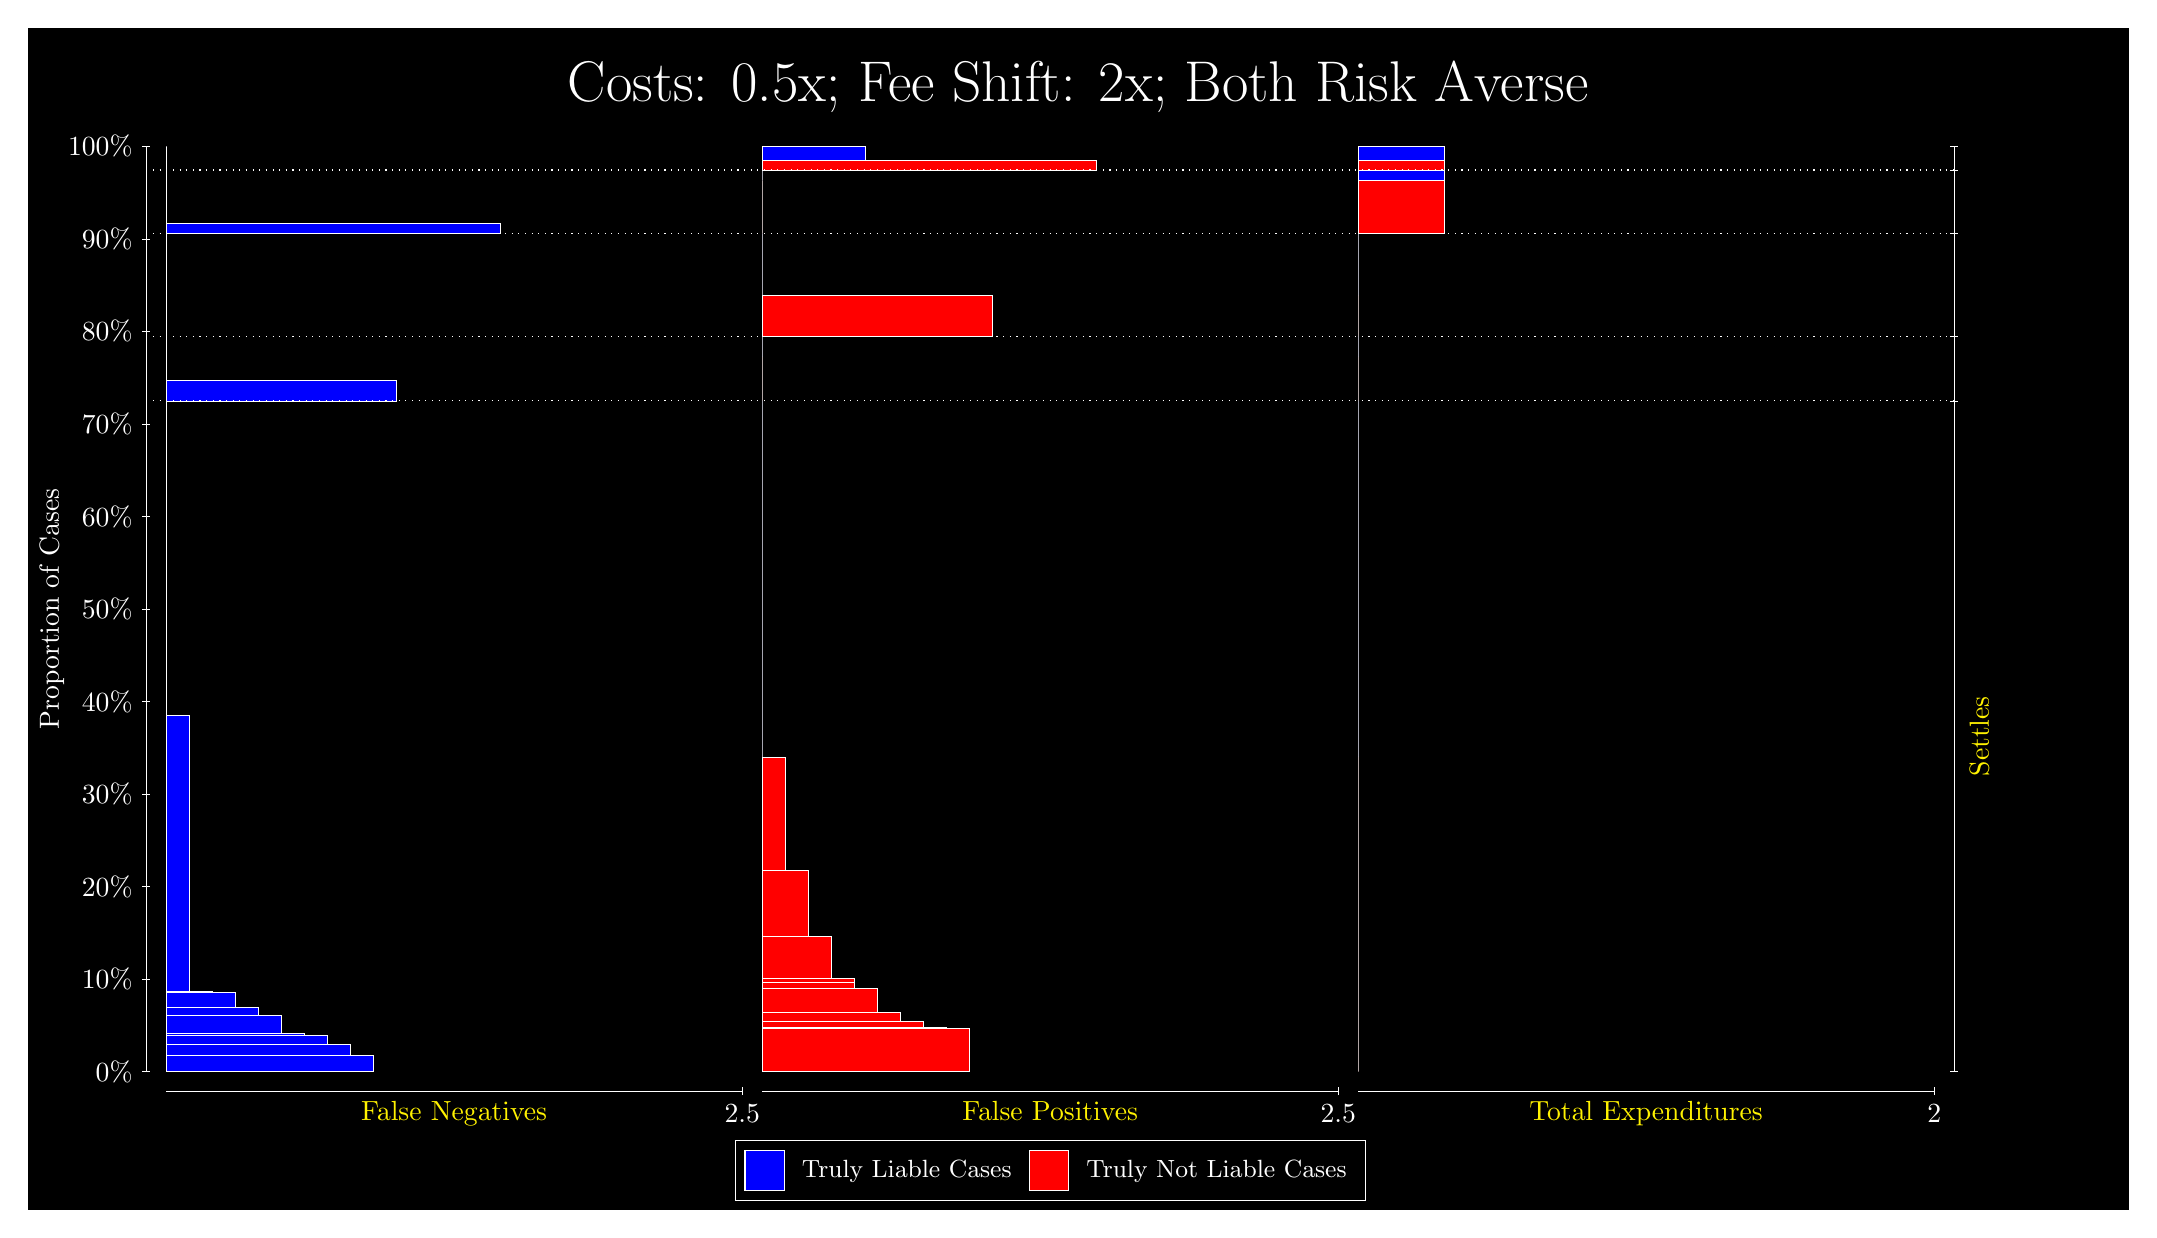
\begin{tikzpicture}
\draw[fill=black] (0,0) rectangle (26.667,15);
\draw[text=white] (0,13.5) rectangle (26.667,15) node[midway] {\huge Costs: 0.5x; Fee Shift: 2x; Both Risk Averse};
\draw[white, very thin] (1.5,1.75) -- (1.5,13.5);
\node[rotate=90, text=white, anchor=center] at (0.3, 7.625) {Proportion of Cases};
\draw[white, very thin] (1.45,1.75) -- (1.55,1.75);
\node[text=white, anchor=east] at (1.45, 1.75) {0\%};
\draw[white, very thin] (1.45,2.925) -- (1.55,2.925);
\node[text=white, anchor=east] at (1.45, 2.925) {10\%};
\draw[white, very thin] (1.45,4.1) -- (1.55,4.1);
\node[text=white, anchor=east] at (1.45, 4.1) {20\%};
\draw[white, very thin] (1.45,5.275) -- (1.55,5.275);
\node[text=white, anchor=east] at (1.45, 5.275) {30\%};
\draw[white, very thin] (1.45,6.45) -- (1.55,6.45);
\node[text=white, anchor=east] at (1.45, 6.45) {40\%};
\draw[white, very thin] (1.45,7.625) -- (1.55,7.625);
\node[text=white, anchor=east] at (1.45, 7.625) {50\%};
\draw[white, very thin] (1.45,8.8) -- (1.55,8.8);
\node[text=white, anchor=east] at (1.45, 8.8) {60\%};
\draw[white, very thin] (1.45,9.975) -- (1.55,9.975);
\node[text=white, anchor=east] at (1.45, 9.975) {70\%};
\draw[white, very thin] (1.45,11.15) -- (1.55,11.15);
\node[text=white, anchor=east] at (1.45, 11.15) {80\%};
\draw[white, very thin] (1.45,12.325) -- (1.55,12.325);
\node[text=white, anchor=east] at (1.45, 12.325) {90\%};
\draw[white, very thin] (1.45,13.5) -- (1.55,13.5);
\node[text=white, anchor=east] at (1.45, 13.5) {100\%};

\draw[white, very thin] (24.457,1.75) -- (24.457,13.5);
\draw[white, very thin] (24.407,1.75) -- (24.507,1.75);
\node[anchor=west] at (24.407, 1.75) {};
\draw[white, very thin] (24.407,10.267) -- (24.507,10.267);
\node[anchor=west] at (24.407, 10.267) {};
\draw[white, very thin] (24.407,11.09) -- (24.507,11.09);
\node[anchor=west] at (24.407, 11.09) {};
\draw[white, very thin] (24.407,12.396) -- (24.507,12.396);
\node[anchor=west] at (24.407, 12.396) {};
\draw[white, very thin] (24.407,13.199) -- (24.507,13.199);
\node[anchor=west] at (24.407, 13.199) {};
\draw[white, very thin] (24.407,13.5) -- (24.507,13.5);
\node[anchor=west] at (24.407, 13.5) {};

\draw[white, very thin, fill=blue] (1.75,1.75) rectangle (4.3848,1.9539);
\draw[white, very thin, fill=blue] (1.75,1.9539) rectangle (4.092,2.092);
\draw[white, very thin, fill=blue] (1.75,2.092) rectangle (3.7993,2.2044);
\draw[white, very thin, fill=blue] (1.75,2.2044) rectangle (3.5065,2.2165);
\draw[white, very thin, fill=blue] (1.75,2.2165) rectangle (3.5065,2.2395);
\draw[white, very thin, fill=blue] (1.75,2.2395) rectangle (3.2138,2.4623);
\draw[white, very thin, fill=blue] (1.75,2.4623) rectangle (2.921,2.5633);
\draw[white, very thin, fill=blue] (1.75,2.5633) rectangle (2.6283,2.7521);
\draw[white, very thin, fill=blue] (1.75,2.7521) rectangle (2.3355,2.7729);
\draw[white, very thin, fill=blue] (1.75,2.7729) rectangle (2.0428,6.2715);
\draw[white, very thin, fill=red] (1.75,6.2715) rectangle (1.75,10.267);
\draw[white, very thin, fill=blue] (1.75,10.267) rectangle (4.6775,10.531);
\draw[white, very thin, fill=red] (1.75,10.531) rectangle (1.75,11.09);
\draw[white, very thin, fill=red] (1.75,11.09) rectangle (1.75,11.61);
\draw[white, very thin, fill=blue] (1.75,11.61) rectangle (1.75,12.396);
\draw[white, very thin, fill=blue] (1.75,12.396) rectangle (5.9949,12.526);
\draw[white, very thin, fill=red] (1.75,12.526) rectangle (1.75,13.199);
\draw[white, very thin, fill=red] (1.75,13.199) rectangle (1.75,13.326);
\draw[white, very thin, fill=blue] (1.75,13.326) rectangle (1.75,13.5);
\draw[white, very thin, fill=red] (9.3189,1.75) rectangle (11.954,2.305);
\draw[white, very thin, fill=red] (9.3189,2.305) rectangle (11.661,2.3133);
\draw[white, very thin, fill=red] (9.3189,2.3133) rectangle (11.368,2.3889);
\draw[white, very thin, fill=red] (9.3189,2.3889) rectangle (11.075,2.507);
\draw[white, very thin, fill=red] (9.3189,2.507) rectangle (10.783,2.806);
\draw[white, very thin, fill=red] (9.3189,2.806) rectangle (10.49,2.8779);
\draw[white, very thin, fill=red] (9.3189,2.8779) rectangle (10.49,2.938);
\draw[white, very thin, fill=red] (9.3189,2.938) rectangle (10.197,3.4681);
\draw[white, very thin, fill=red] (9.3189,3.4681) rectangle (9.9044,4.3098);
\draw[white, very thin, fill=red] (9.3189,4.3098) rectangle (9.6116,5.7451);
\draw[white, very thin, fill=blue] (9.3189,5.7451) rectangle (9.3189,10.267);
\draw[white, very thin, fill=red] (9.3189,10.267) rectangle (9.3189,10.826);
\draw[white, very thin, fill=blue] (9.3189,10.826) rectangle (9.3189,11.09);
\draw[white, very thin, fill=red] (9.3189,11.09) rectangle (12.246,11.61);
\draw[white, very thin, fill=blue] (9.3189,11.61) rectangle (9.3189,12.396);
\draw[white, very thin, fill=red] (9.3189,12.396) rectangle (9.3189,13.069);
\draw[white, very thin, fill=blue] (9.3189,13.069) rectangle (9.3189,13.199);
\draw[white, very thin, fill=red] (9.3189,13.199) rectangle (13.564,13.326);
\draw[white, very thin, fill=blue] (9.3189,13.326) rectangle (10.636,13.5);
\draw[white, very thin, fill=red] (16.888,1.75) rectangle (16.888,5.7451);
\draw[white, very thin, fill=blue] (16.888,5.7451) rectangle (16.888,10.267);
\draw[white, very thin, fill=red] (16.888,10.267) rectangle (16.888,10.826);
\draw[white, very thin, fill=blue] (16.888,10.826) rectangle (16.888,11.09);
\draw[white, very thin, fill=red] (16.888,11.09) rectangle (16.888,11.61);
\draw[white, very thin, fill=blue] (16.888,11.61) rectangle (16.888,12.396);
\draw[white, very thin, fill=red] (16.888,12.396) rectangle (17.986,13.069);
\draw[white, very thin, fill=blue] (16.888,13.069) rectangle (17.986,13.199);
\draw[white, very thin, fill=red] (16.888,13.199) rectangle (17.986,13.326);
\draw[white, very thin, fill=blue] (16.888,13.326) rectangle (17.986,13.5);
\draw[white, dotted] (1.5,10.267) -- (24.457,10.267);
\draw[white, dotted] (1.5,11.09) -- (24.457,11.09);
\draw[white, dotted] (1.5,12.396) -- (24.457,12.396);
\draw[white, dotted] (1.5,13.199) -- (24.457,13.199);
\draw[white, very thin] (1.75,1.5) -- (9.0689,1.5);
\node[text=yellow, anchor=north] at (5.4094, 1.5) {False Negatives};
\draw[white, very thin] (9.0689,1.45) -- (9.0689,1.55);
\node[text=white, anchor=north] at (9.0689, 1.45) {2.5};

\draw[white, very thin] (9.3189,1.5) -- (16.638,1.5);
\node[text=yellow, anchor=north] at (12.978, 1.5) {False Positives};
\draw[white, very thin] (16.638,1.45) -- (16.638,1.55);
\node[text=white, anchor=north] at (16.638, 1.45) {2.5};

\draw[white, very thin] (16.888,1.5) -- (24.207,1.5);
\node[text=yellow, anchor=north] at (20.547, 1.5) {Total Expenditures};
\draw[white, very thin] (24.207,1.45) -- (24.207,1.55);
\node[text=white, anchor=north] at (24.207, 1.45) {2};

\node[text=yellow, centered, rotate=90] at (24.777, 6.0083) {Settles};





\draw (12.978300999999998,1.5) node[draw=none] (baseCoordinate) {};
\begin{scope}[align=center]
        \matrix[scale=0.5, draw=white, below=0.5cm of baseCoordinate, nodes={draw}, column sep=0.1cm]{
            \node[rectangle, draw, minimum width=0.5cm, minimum height=0.5cm, fill=blue] {}; &
            \node[draw=none, font=\small, text=white] (B) {Truly Liable Cases}; &
            \node[rectangle, draw, minimum width=0.5cm, minimum height=0.5cm, fill=red] {}; &
            \node[draw=none, font=\small, text=white] (B) {Truly Not Liable Cases}; \\
            };
\end{scope}

\end{tikzpicture}
\end{document}